\section{Image Processing}

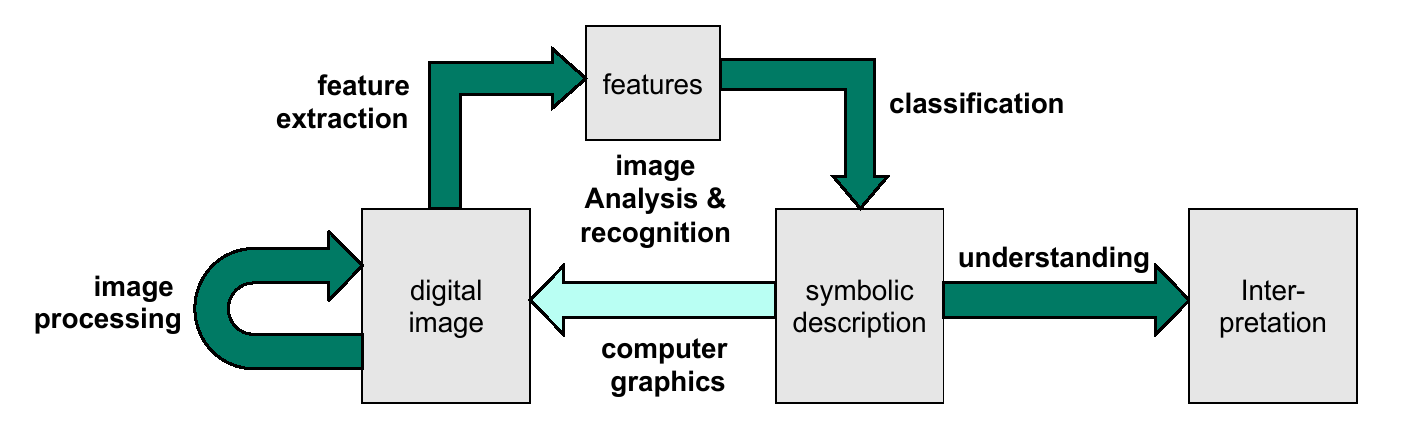
\includegraphics[width=\textwidth]{02_image_disciplines}

\begin{description}
		\item[Image digitalization] Sample to produces pixels, quantize to determine pixel values
		\item[Representation of digital image] Usually as 2D grid.
				Alternatively: Pyramid, with each layer a different resolution.
		\item[Color modes] Direct colour (channels) vs indexed colour (colour map)
		\item[Color spaces] Many different ones
		\item[Quantization] Determine range of pixel values
\end{description}


\subsection{Compression}

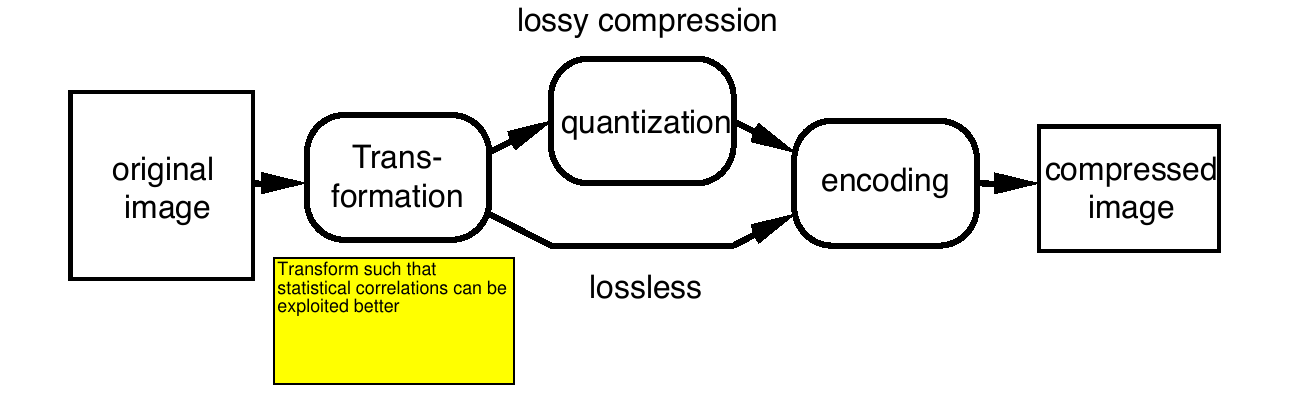
\includegraphics[width=\textwidth]{02_compression}

\begin{itemize}
		\item Lossy vs lossless
		\item Entropy $H(x) = - \sum_{i=1}^n p(i) \log_2(p(i))$. Maximal $H(x)
				= \log_2(n)$ iff all states equally likely (eg uniform noise).
				Minimal $H(x) = 0$ if only one state.
		\item Example: Huffman code, quadtree (recursively partition into four
				quadrants until you get homogenous space)
\end{itemize}

\subsection{Processing operations}

\begin{description}
		\item[Point operation] $z = f(u)$, output depends only on corresponding
				pixel of input. Eg colour inversion, threshold, logical
				combinations.
		\item[Local operation] Each output pixel $(x, y)$ depends on
				neighbourhood $V(x, y)$ of source. Eg convolution operations,
				morphological filters, statistical filters.
		\item[Global operation] Output pixel depends on all pixels of source.
\end{description}

\subsubsection{Convolution}

Mathematical operation of two functions $f$, $g$ producing a third function
defined as (for two dimensions):
\begin{align*}
		f(x, y) \cdot g(x, y) = \int_{- \infty}^{\infty} \int_{-
		\infty}^{\infty} f(\alpha, \beta) \cdot g(x - \alpha, y - \beta)
		d\alpha d\beta
\end{align*}

Discrete case of image $I$ with kernel $k$:
\begin{align*}
		(k \cdot I)[x, y] = \sum_{u = -m}^{m} \sum_{v = -n}^n k[u, v] \cdot I[x
		- u, y - v]
\end{align*}

Kernel is a form of weight given to each pixel the corresponding position. NB
horizontall and veritically flipped in this definition.

\begin{itemize}
		\item Convolution is linear, commutative, associative and shift-independent
		\item Convolution separable iff $k = k_x \cdot k_y$. Reduces complexity
				from $O(m \cdot n \cdot w \cdot h)$ to $O((m + n) \cdot w \cdot
				h)$

		\item Can be used to implement e.g. edge detection, gaussian smoothing,
				min/max/median filter
\end{itemize}

\subsubsection{Spatial vs frequency domain}

\begin{itemize}
		\item Can be toggled between with direct (spaitla -> frequency) and
				inverse (frequency -> spatial) fourier transform.
\end{itemize}
